% coding:utf-8

\section{Recovery Time}

\subsection{Messaufbau}
\begin{frame}
\frametitle{Messaufbau}
\begin{figure}[h!]
  \begin{circuitikz}[scale=1]\draw
    % (0,0) node[anchor=east] {GND}
    % (0,0) node[anchor=east] {GND}
    % (0,0) to[short, o-*] (2,0)
    (0,0) to[V, l=V$_\text{q}$, ] (0,4)
    (2,4) to[R=$100\Omega$, -*] (2,2)
    (2,2) to[D, l=D, *-*] (2,0)
    (0,4) to[short, -*] (2,4)
    (0,0) to[short, -*] (2,0)
    (2,4) to[short, *-o] (4,4)
    (2,2) to[short, *-o] (4,2)
    (2,0) to[short, *-o] (4,0)
    (4,4) node[anchor=west] {CH1}
    (4,2) node[anchor=west] {CH2}
    (4,0) node[anchor=west] {GND}
%     (6,2) node[anchor=west] {KO}
    (2,0) node[ground] {};
  \end{circuitikz}
  \caption{Messschaltung}
\end{figure}
\end{frame}

\subsection{Erwartung}
\begin{frame}
\frametitle{Erwartung}
  \begin{itemize}
    \item 1N4007: 30$\mu$s
    \item 1N4148: 4ns
    \item BAT81: keine Recovery Time
  \end{itemize}
\end{frame}

\subsection{Ergebnisse}
\subsubsection{1N4007}
\begin{frame}
\frametitle{Ergebnisse -- 1N4007}
  \begin{figure}
    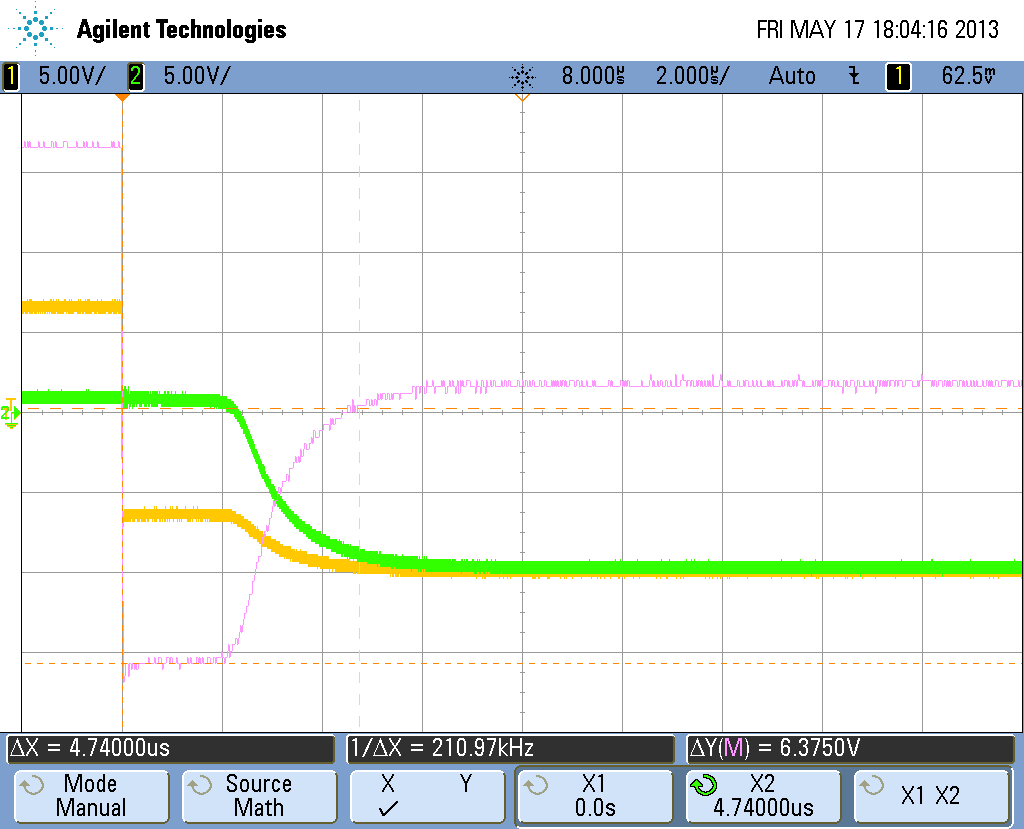
\includegraphics[width=0.7\columnwidth]{fig/scope_18.png}
    \caption{1N4007}
  \end{figure}
\end{frame}

\subsubsection{1N4148}
\begin{frame}
\frametitle{Ergebnisse -- 1N4148}
  \begin{figure}
    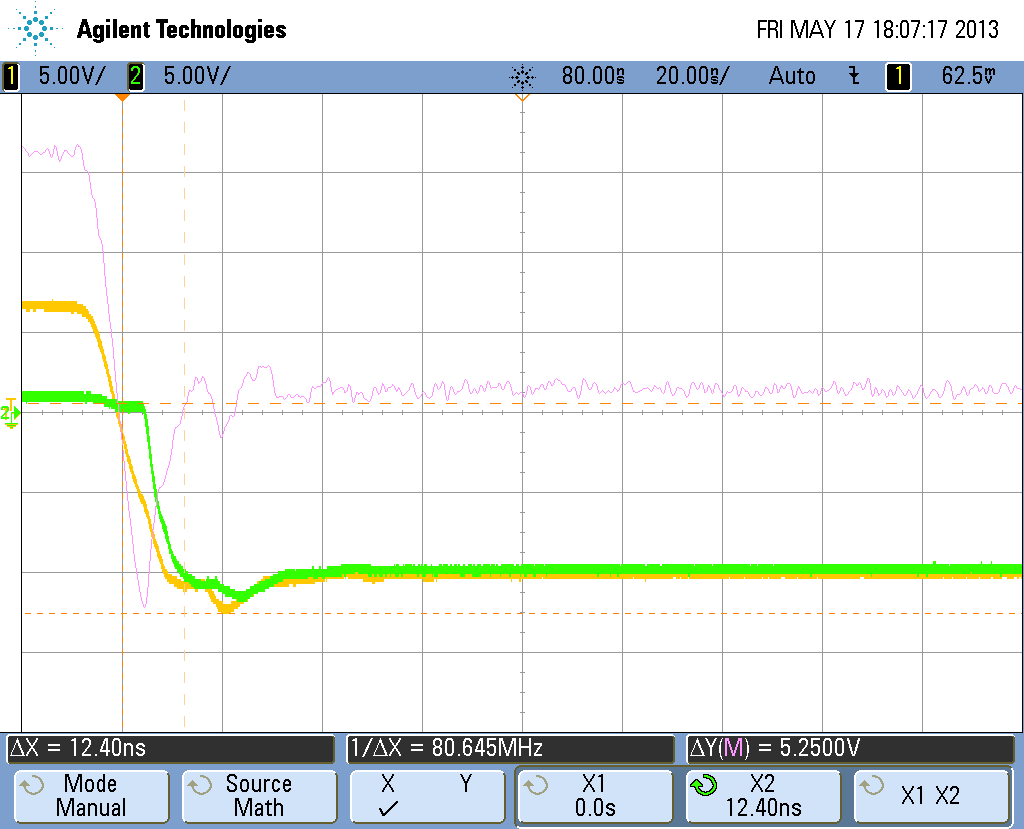
\includegraphics[width=0.7\columnwidth]{fig/scope_19.png}
    \caption{1N4148}
  \end{figure}
\end{frame}

\subsubsection{BAT81}
\begin{frame}
\frametitle{Ergebnisse -- BAT81}
  \begin{figure}
    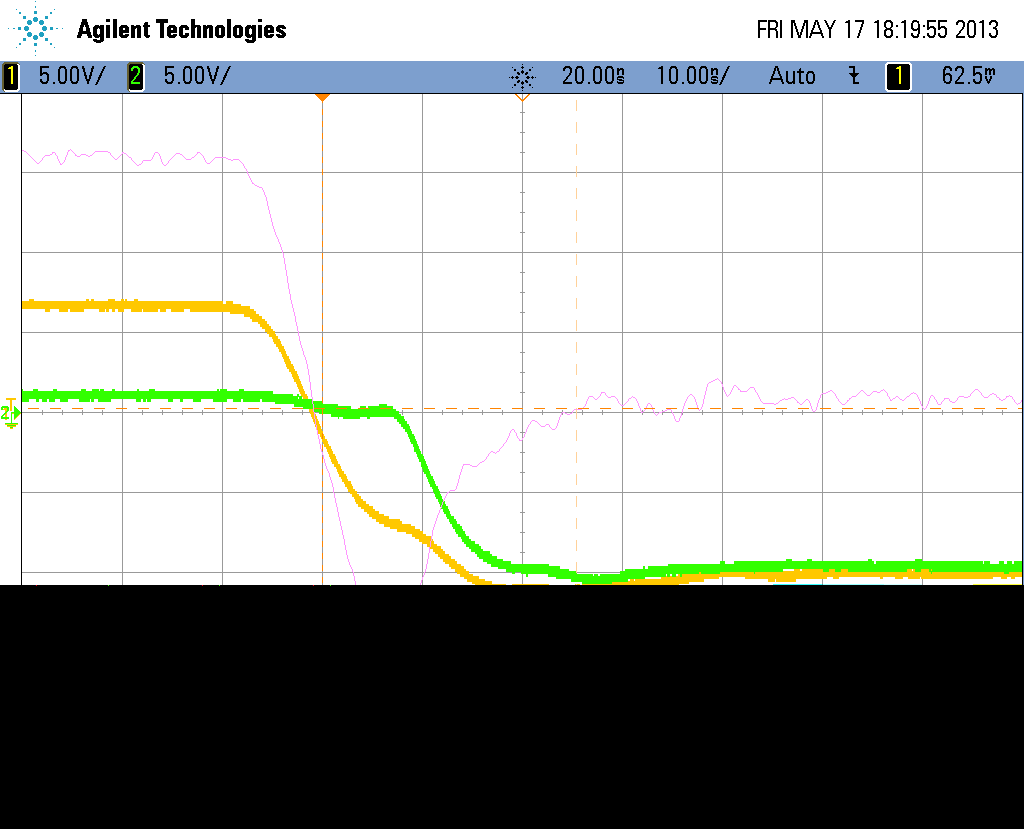
\includegraphics[width=0.7\columnwidth]{fig/scope_20_2.png}
    \caption{BAT81}
  \end{figure}
\end{frame}

\subsection{Fazit}
\begin{frame}
\frametitle{Fazit}
  \begin{itemize}
    \item 1N4148 ist viel schneller als 1N4007
    \item BAT81 ist langsamer als 1N4148
  \end{itemize}
\end{frame}
